\chapter{nEDM measurement at PSI}
\label{ch:nedm-at-psi-apparatus}

% \section{The collaboration}
In the Paul Scherrer Institute (PSI) in Villigen, Switzerland, a collaboration has been founded to perform an nEDM measurement there. The experiment had been planned in two stages. In the first one, the apparatus used in the ILL experiment was moved to PSI, where it was installed to benefit from a new, highly intense source of ultracold neutrons~\cite{Lauss2014}. The first stage finished in Autumn 2017, after having collected enough statistics to set the world's best limit (Fig.\,\ref{fig:nEDM_accumulated_sensitivity}). As of Spring 2018 the data analysis is still ongoing.

\begin{figure}
  \centering
  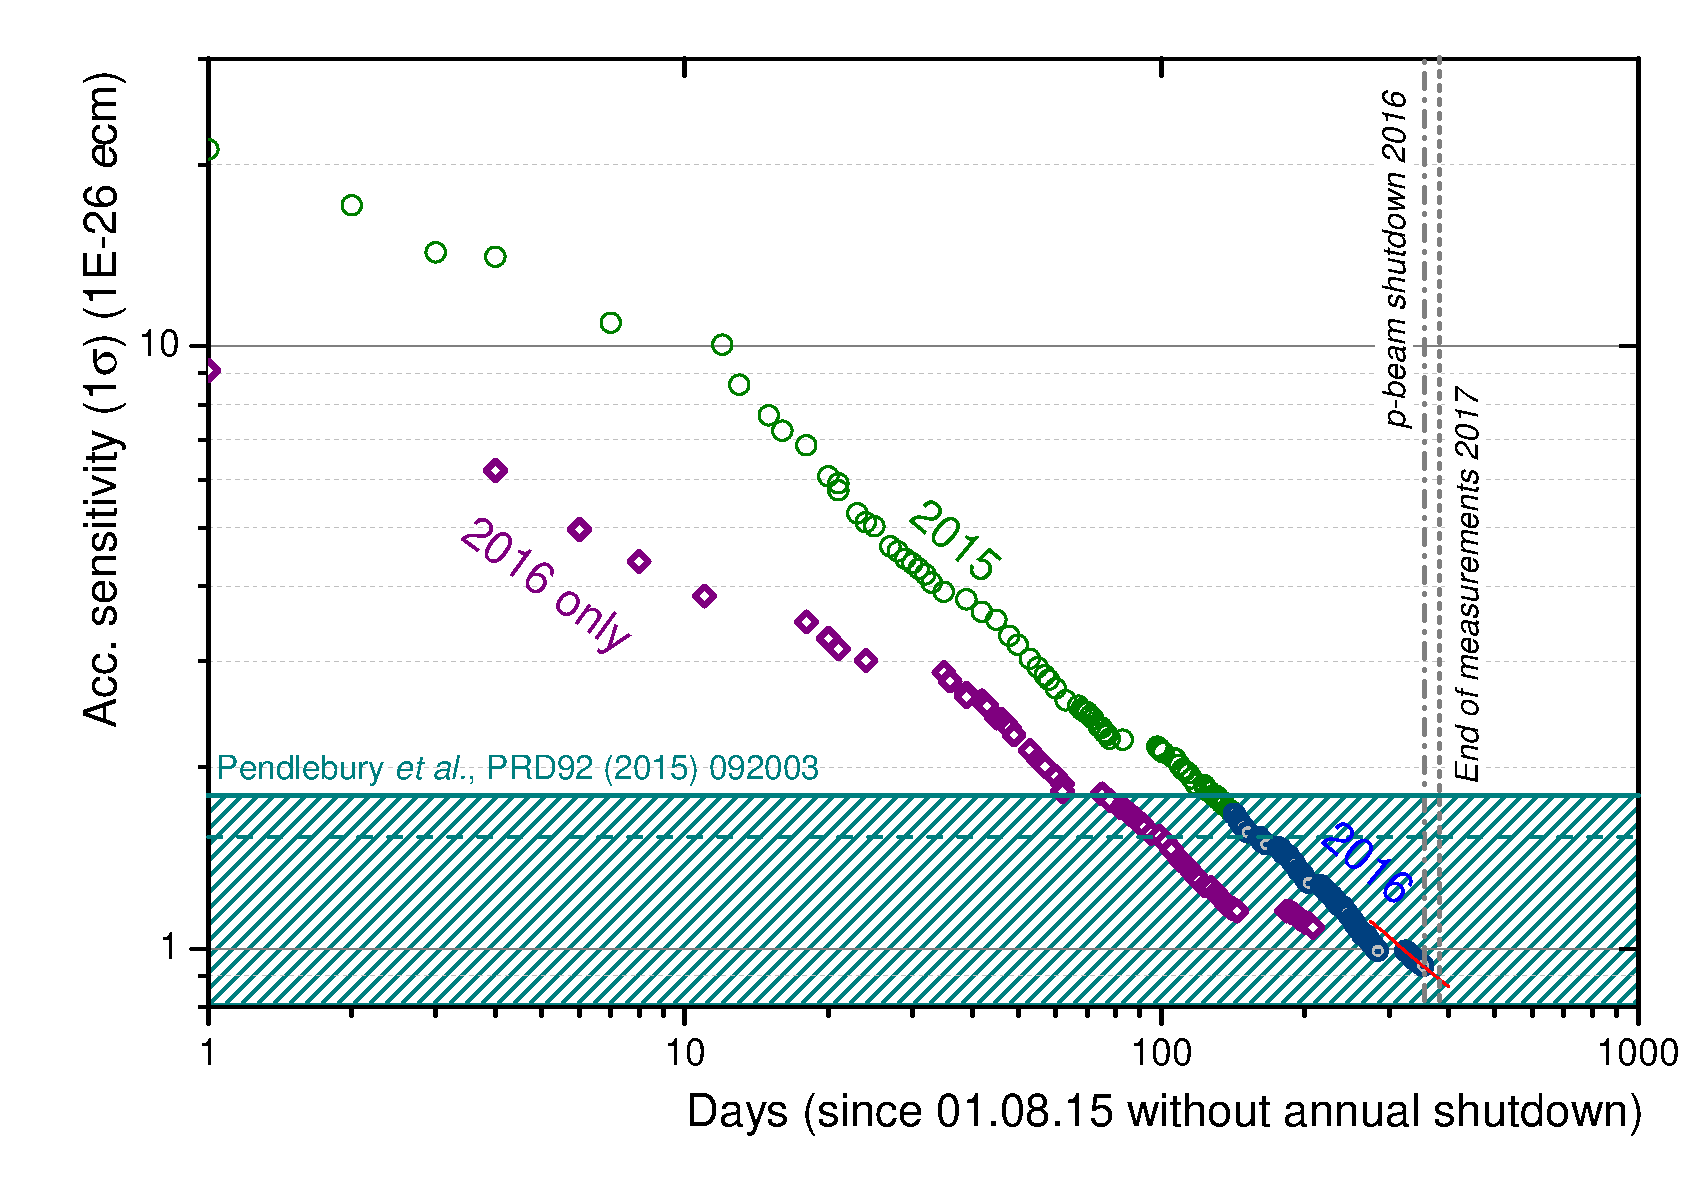
\includegraphics[width=\linewidth]{gfx/nEDMatPSI/accumulated_sensitivity.pdf}
  \caption{The accumulated statistical sensitivity of the nEDM-at-PSI experiment. The sensitivity of the data collected in 2015 is shown in green, of 2015 and 2016 in blue, and only 2016 in violet. The dashed region marks the yet unexplored area below the best limit~\cite{Pendlebury2015}. Courtesy of Dr.\ Philipp Schmidt-Wellenburg.}\label{fig:nEDM_accumulated_sensitivity}
\end{figure}

Already in the first stage the apparatus underwent numerous improvements, leaving only few parts of the original. The improvements were part of the research and development plan for the second stage, a newly built apparatus called n2EDM\@. The new experiment, designed by the personnel experienced with running, modifying and improving the first stage, would have the goal of exploring the \SI{e-27}{\elementarycharge\centi\meter} range.


\section{The apparatus}
This work focuses on the stage-one apparatus. It employed the Ramsey method with ultracold neutrons stored for the time of the precession. The neutrons, produced in the PSI source, were guided with a pipe system into a storage chamber, where they underwent the Ramsey procedure. The polarisation was then measured by letting the neutrons fall into a spin-state--sensitive neutron detector. A diagram of the system is shown in Fig.\,\ref{fig:nEDM_scheme}.

\begin{figure}
  \centering
  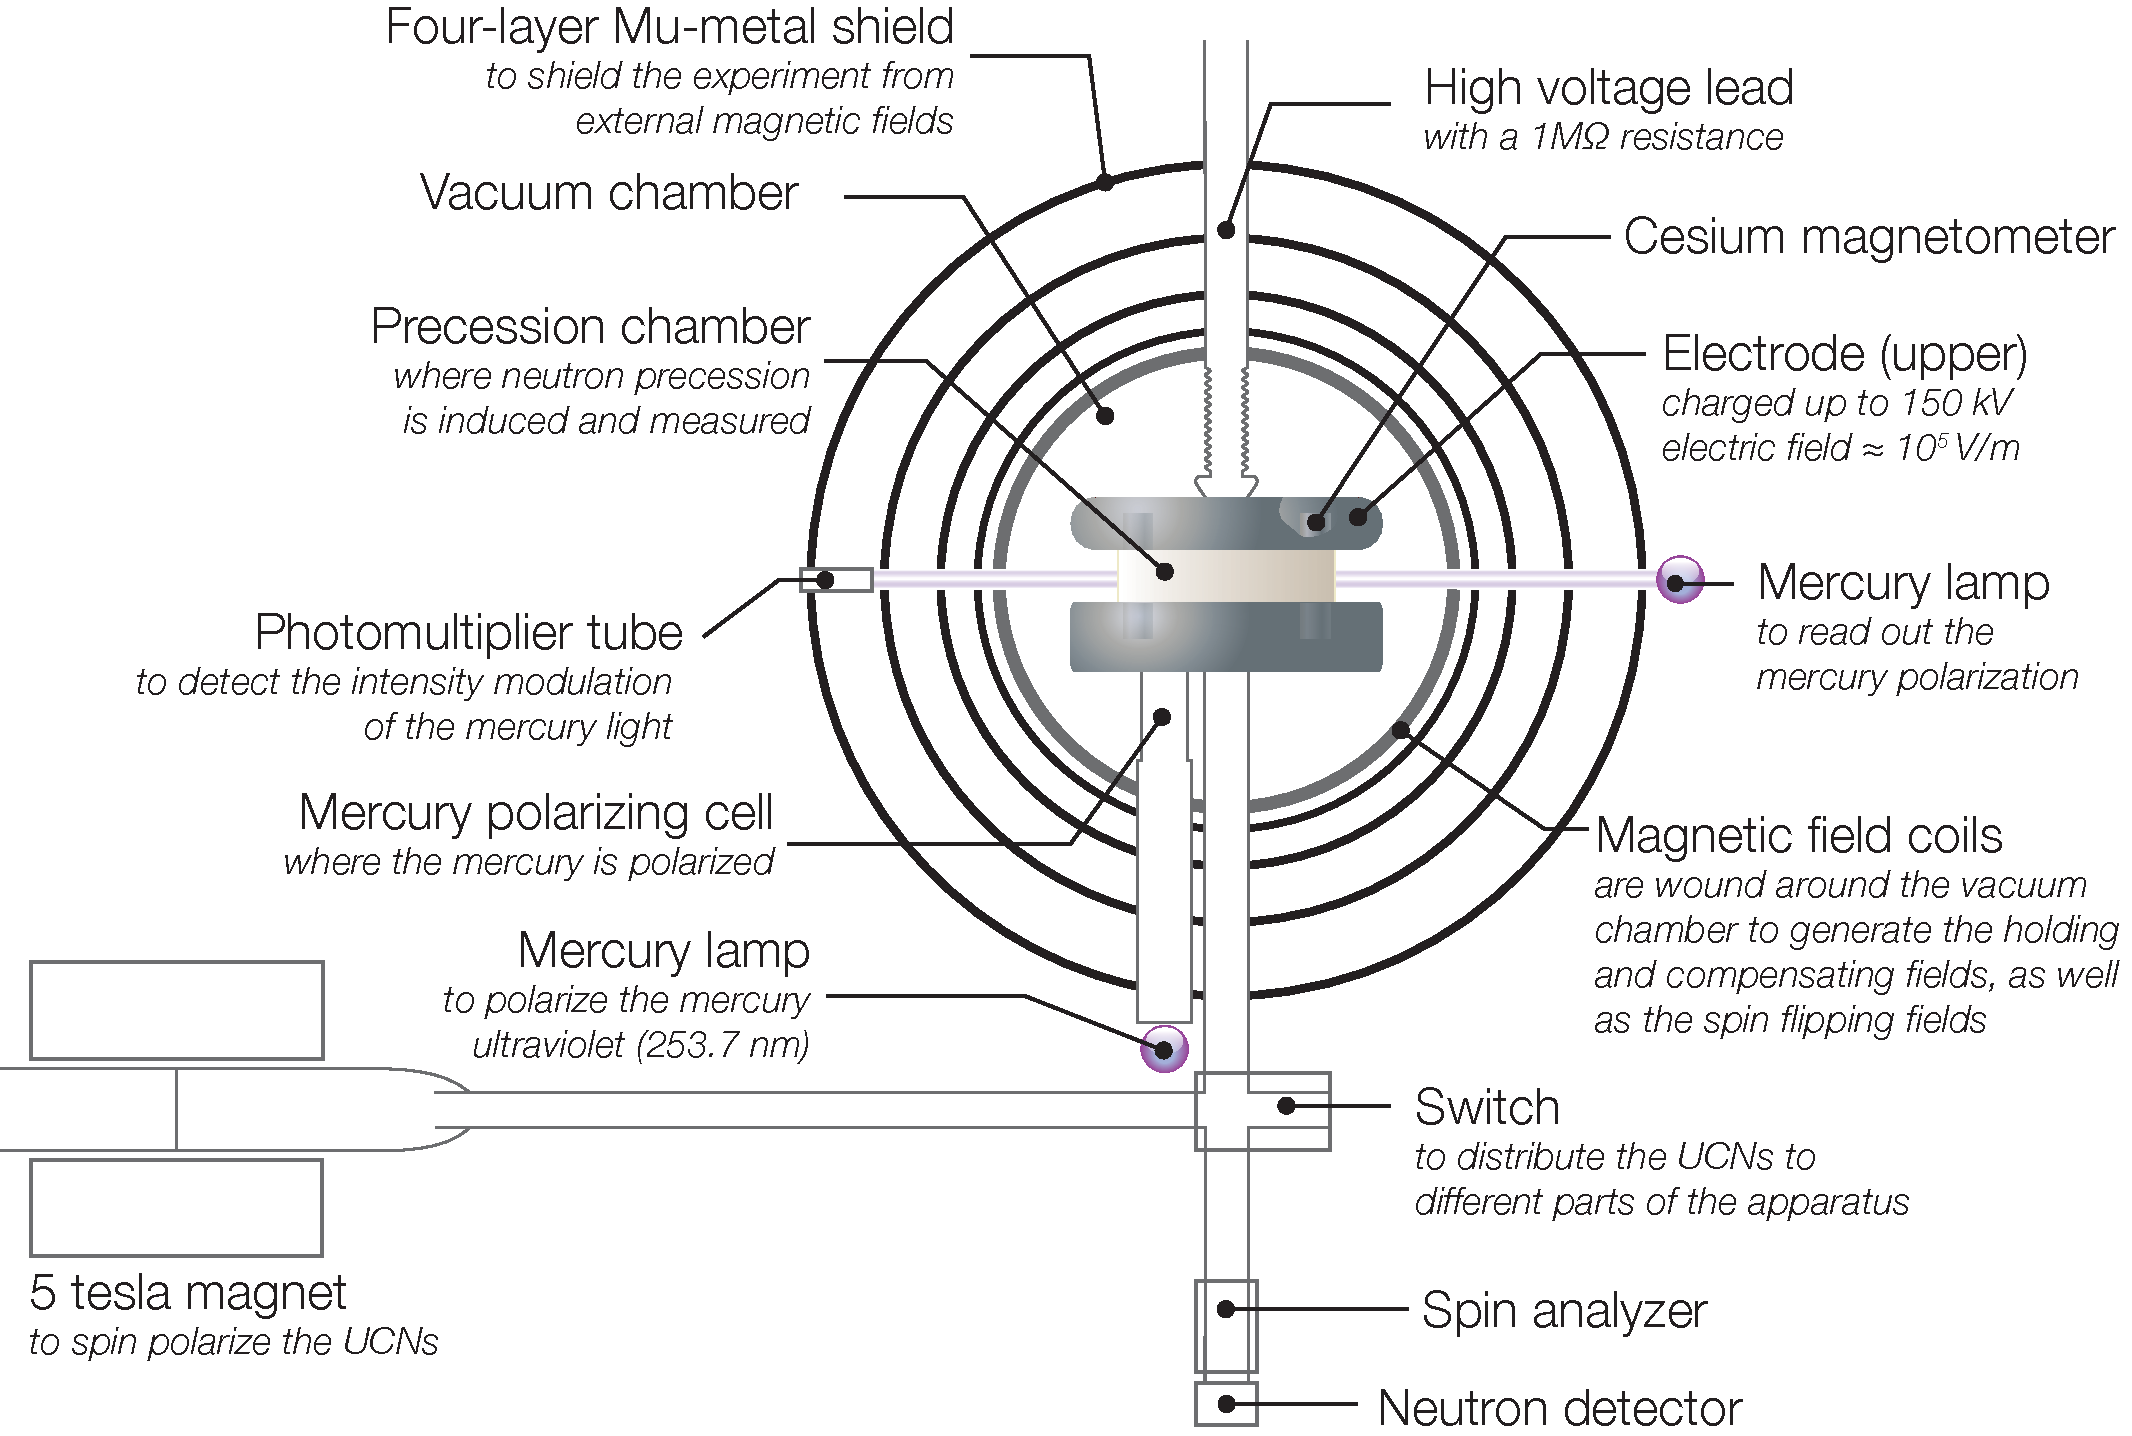
\includegraphics[width=\linewidth]{gfx/nEDMatPSI/apparatus-cartoon-main-and-sub-labels.pdf}
  \caption{The scheme of the nEDM-at-PSI apparatus. \note{Whom to credit for the image? Make my own? No\ldots} \note{Make the labels in the Palatino font to match the text.}}\label{fig:nEDM_scheme}
\end{figure}

A single measurement cycle was triggered by a pulse of ultracold neutrons incoming from the PSI source, from which the neutrons were guided in metal-coated glass pipes. First, they were polarised by passing through a five-tesla magnet. Then, a rotary three-way valve, called the switch, directed the neutrons upwards into a vacuum tank, where they filled a \SI{12}{\centi\meter} high cylindrical precession chamber. The chamber was sandwiched between high-voltage electrodes, charged to \SI{132}{\kilo\volt}, which created an electric field in the chamber. The whole stack was submerged in a \SI{1}{\micro\tesla} vertical magnetic field $B_0$. Once the neutrons filled the cylinder, the entrance was shut and the particles were stored for around \SI{200}{\second} to undergo the Ramsey procedure.

\marginpar{At the nEDM experiment at psithe neutrons were dropped into two-armed detector, capable of counting both spin states simultaneously~\cite{Afach2015USSA}.}
First, a pulse of rotating transverse field was applied, with its amplitude and length tuned so that the neutrons' spins flip from the vertical orientation, along the $B_0$ field, to the horizontal plane (a $\uppi/2$ pulse).
This set the spins into a Larmor precession.
After \SI{180}{\second} a second pulse, in phase with the first one, was applied. Then the chamber's entrance was opened, and the neutrons were allowed to fall through the switch and a spin analyser into the neutron detector.


Many of rest of the components, in fact---the majority, is either providing a stable magnetic field environment in the precession chamber or measuring the field.




\section{Magnetic fields}
\marginpar{The exact attenuation factor of the shield depended on the direction and varied from 1600 to 13300~\cite{Komposch2017}.}
The most important method of stabilising the magnetic field is passive shielding. The vacuum tank, with the precession chamber in it, was covered by four layers of highly permeable material, called mu-metal.
Each layer attenuated the magnetic field changes by a factor of approximately ten. The high magnetic permeability of the mu-metal makes the magnetic field much rather go inside the metal and around the volume it encloses, than to penetrate into the volume. 
%Even though mu-metal provided excellent shielding properties, as a ferromagnetic it distorts the field both outside and inside the shield. Also it had to be regularly demagnetised.

Inside the shield, on the vacuum chamber, there were a number of coils wound. 
% The main magnetic field $B_0$ was produced by a cos-theta coil.
\marginpar{In an ensemble precessing in an inhomogenous field, members in different places precess at slightly different rates. This leads to depolarisation by the loss of coherence.}
Besides the one producing the main magnetic field $B_0$, there were numerous others, producing fields of various shapes.
Those were, on one hand, used to homogenise the field, which reduced the depolarisation rate of the neutrons. On the other hand, they were used to deliberately apply vertical gradients $\partial_z B_0$; Operating in different gradients was part of the measurement procedure and is explained later in this chapter.

The stability of the field inside the shield was in the picotesla range. The remaining variations were measured and corrected for, primarily with a mercury-based magnetometer~\cite{FertlThesis,Komposch2017}. Below the precession chamber there was a cell containing a vapour of polarised $^{199}$Hg atoms, which was released into the precession chamber once it had been filled with neutrons.
\marginpar{In the \SI{1}{\micro\tesla} $B_0$ field the precession frequencies of neutrons and $^{199}$Hg atoms are approximately \SI{30}{\hertz} and \SI{8}{\hertz}, respectively. The respective spin-flip pulses affect the other species only very slightly.}
There, a dedicated $\uppi/2$ pulse of a rotating transverse magnetic field started their coherent precession, which was read on-line optically. A mercury discharge lamp shone a circularly polarised light through the precession chamber onto a photomultiplier tube. As the mercury atoms' photon-capture cross-section depended on the phase of the precession, the transparency of the chamber to the polarised light oscillated at the mercury's Larmor frequency. The oscillating signal of the photomultiplier was then analysed to estimate its frequency, proportional to the $B_0$ field, as averaged by the mercury atoms.

The mercury magnetometer may seem an ideal measure to correct the neutron measurement for the drifts of the magnetic field, as the two species filled exactly the same volume (hence it is often called a \emph{comagnetometer}). Only, they did not measure the exact same field. The ultracold neutrons were slow enough to be affected by the gravity, which shifted their centre of mass around \SI{2.4}{\milli\meter} relative to the warm, homogeneous mercury vapour~\cite{Afach2014magmoment}. In a presence of a vertical gradient, the two species saw different fields. A detailed discussion of additional systematic effects related to this magnetometer can be found in~\cite{Afach2014magmoment}.

A way to measure vertical gradients, as well as other high-order components of the magnetic field, was provided by an array of Caesium magnetometers~\cite{Groeger2005}. These sensors were located inside the electrodes---seven in the top one, nine in the bottom one. Each magnetometer was a cell filled with Caesium vapour, through which a circularly polarised light, delivered with a light guide, shone at \SI{45}{\degree} inclination angle. The light simultaneously polarised the atoms and, as it met a surface of a photodiode behind the cell, probed their precession. A coil wound around the cell, axial with the light beam, was driven in a feedback loop with the diode's signal to resonantly drive the Larmor precession. Even though the magnetometers measured only the magnitude of the magnetic field, they provided information about the higher-order components of the field thanks to their distribution around the chamber. For example, one could na\"\i vely estimate the vertical gradient $\partial_z B_z$ by evaluating the average readings of the sensors in each electrode, taking the difference and dividing by the vertical separation. Actually, the high-order field terms, including the vertical gradient, were obtained by fitting a second-order parametrization of the magnetic field to the readings of the sensors~\cite{WurstenThesis}.

In the next section we describe how all these components came together to perform a measurement of the electric dipole moment of the neutron.



\section{Measurement procedure}
\label{sec:measurement_procedure}

\begin{figure}
  \centering
  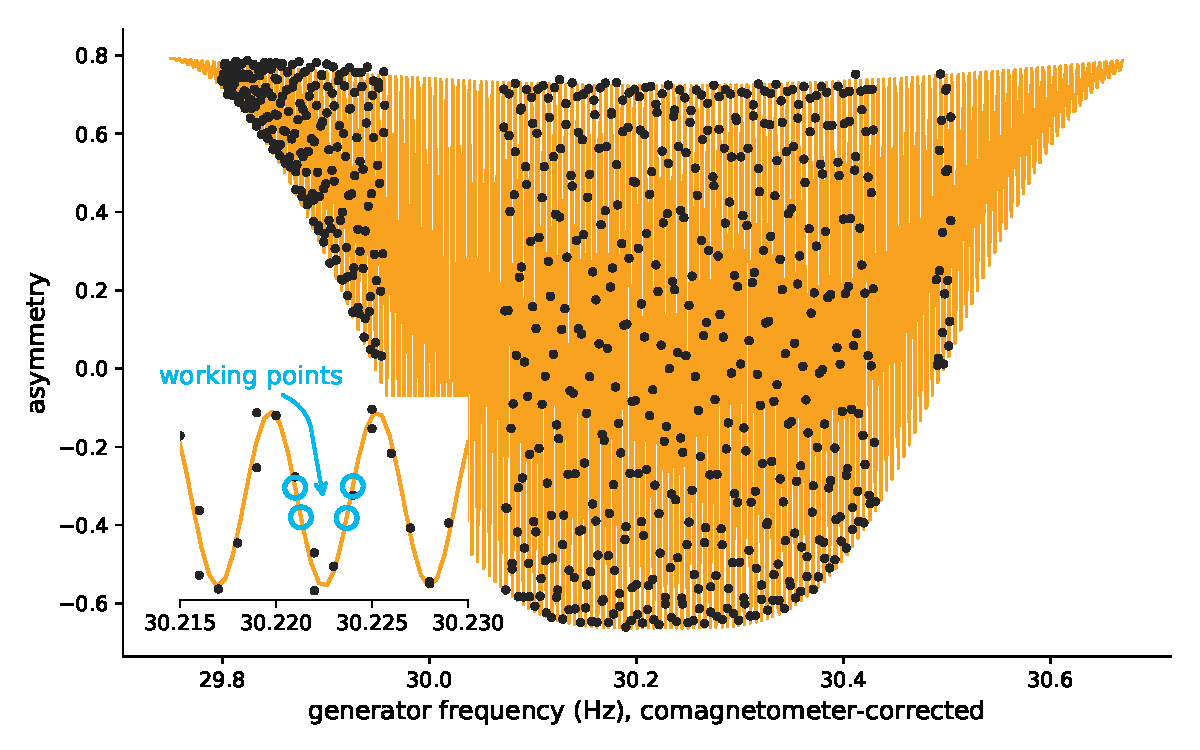
\includegraphics[width=\linewidth]{gfx/nEDMatPSI/ramsey_scan.pdf}
  \caption{A scan of the Ramsey resonance curve in the nEDM experiment at the PSI\@. The asymmetry (the difference between spin-up and spin-down counts, normalised to their sum) is measured as the function of the detuning of the spin-flip generator's frequency. The black points depict the measured points, the orange line is the fit of the theoretical model. In the inset, the central fringe is enlarged and the working points are marked, which is where the experiment took data during normal operation. The generator frequency has been corrected with the $^{199}$Hg comagnetometer using the formula $\nu_\text{generator} / \nu_\text{Hg} \times \overline{\nu_\text{Hg}}$, where $\overline{\nu_\text{Hg}}$ is the average over the scan. The resonance curve was scanned in runs 12666 and 12678.}\label{fig:ramsey_scan}
\end{figure}

Recall the Ramsey method (Fig.\,\ref{fig:nEDM_Ramsey_principle}). Two coherent pulses of a transverse oscillating field are applied to an ensemble of polarised neutrons, with a period of free precession in between. Measuring the polarisation after the second pulse as the function of the frequency of the transverse field yields a resonance curve. The curve measured in the PSI experiment is reproduced in Fig.\,\ref{fig:ramsey_scan}. Comparing it with Ramsey's original curve (Fig.\,\ref{fig:nEDM_Ramsey_original_curve}) summarises fifty years of progress in measuring the electric dipole moment of the neutron.

In the normal operation not the whole curve was sampled, but only the region most sensitive to the position of the central fringe---its steepest slope. In Fig.\,\ref{fig:ramsey_scan} the four \emph{working points} are marked, which the experiment was programmed to aim at. Assuming all the data are taken in this most sensitive region, the sensitivity for the nEDM is~\cite{FertlThesis}:
\begin{equation}
  \label{eq:nEDM_sensitivity}
  \sigma(d_\text{n}) = \frac{\hbar}{ 2 \alpha E T \sqrt{N} } \quad ,
\end{equation}
where $\alpha$ is the relative height of the curve ($\alpha = 1$ means the curve spanning from $-1$ to $1$ in asymmetry), $E$ is the strength of the electric field, $T$ is the duration of the free precession (\SI{180}{\second}, its inverse is the width of the fringes), and $N$ is the counting statistics. It is the statistical limit on the sensitivity, the value obtained from the analysis is expected be slightly worse.

Each cycle of the experiment, filling in the neutrons, performing the Ramsey procedure and counting them, sampled one of the working points on the resonance curve. Assuming that the only parameter of the curve that changed between the cycles was the position of the resonance (due to drifts of the field), one could estimate the position of the central fringe, the neutron precession frequency $\nu_\text{n}$ for each cycle. In other words, the neutrons were a very accurate magnetometer operating on a cycle basis.
% The resonance frequency $f_n^{\,0}$ is determined with a fit of the resonance curve. Because the points are probed one after another, it is only possible after a set of data points, \emph{cycles}, have been measured. In order to extract the neutron precession frequency for each individual \emph{cycle}, one assumes that the only parameter of the resonance curve that varies on a cycle--to--cycle basis is the position of the resonance. With this assumption the shape of the curve, fitted to the whole set of \emph{cycles}, is used to calculate back the resonant frequency in each \emph{cycle} of the set.

Naturally, measuring the magnetic field with the neutrons was not the goal. It was the much, much smaller, if any, effect of the electric field on the precession frequency that the experiment was after. To even out the variations in $\nu_\text{n}$ due to fluctuations of the magnetic field its ratio to the frequency of the comagnetometer's mercury atoms $\nu_\text{Hg}$ was used instead:
\marginpar{This correction was already included in the depiction of the resonance curve in Fig.\,\ref{fig:ramsey_scan}.}
\begin{equation}
  \label{eq:Rdefinition}
  R \equiv \frac{\nu_\text{n}}{\nu_\text{Hg}} = \frac{\mu_\text{n}}{\mu_\text{Hg}} \pm \left( d_\text{n} \mp \frac{\mu_\text{n}}{\mu_\text{Hg}} \, d_\text{Hg} \right) \frac{2 E}{ h  \nu_\text{Hg}} + \Delta \ ,
\end{equation}
where the signs correspond to the parallel and anti-parallel configuration of the magnetic and electric fields. (The derivation of the formula can be found in App.\,\ref{ch:R_derivation_appendix}.)
It is immediately visible that $R$ is sensitive to $d_\text{n}$ just as $\nu_\text{n}$, but the fluctuations due the changes of the magnetic field are suppressed.
\marginpar{$R$ is actually sensitive to $d_\text{n} - \frac{\mu_\text{n}}{\mu_\text{Hg}} \, d_\text{Hg}$, but it has been measured that $|d_\text{Hg}| < \SI{7.4e-30}{\elementarycharge\centi\meter}$~\cite{PhysRevLett.116.161601}.}
$\Delta$ encapsulates all higher-order terms and systematic effects. In particular, the already mentioned effect due to the gravitational sag of the neutrons' population, relative to the geometrical centre of the chamber, in combination with a vertical gradient of the magnetic field.
% Together with the UCNs there is a polarised $^{199}$Hg gas precessing. Its precession is monitored with light, allowing for direct determination of the $^{199}$Hg Larmor frequecy and thus the magnetic field strength. In order to cancel the first-order magnetic field changes one looks at the value:
% \begin{equation}
%   R := f_n / f_{Hg} \ .
% \end{equation}
% However, the UCNs are cold enough to have their centre of mass shifted downwards a few centimeters by the gravity. The $^{199}$Hg gas, being much hotter then the UCNs, fills the precession volume homogeneously. In a presence of a vertical magnetic field gradient this causes the two species to see different magnetic fields.

% The largest effect in $\Delta$ has to do with the gradient of the magnetic field. The neutrons and mercury did not sample exactly the same field. The mercury vapour was at room temperature and filled the precession volume homogeneously. At the same time, the ultracold neutrons had an energy of only around \SI{300}{\nano\electronvolt}, while their gravitational potential is $m_\text{n} = \SI{102}{\nano\electronvolt\per\meter}$ steep~\cite{Zenner2013}. In effect, they filled, and sampled, the bottom of the chamber more then the top. The difference between centres of masses of the mercury and the neutrons was around \SI{4}{\mili\meter}


To get the $d_n$ estimate the electric field needed to be modulated. The experiment automatically reversed the polarisation of the electric field every 72 cycles. In between the two polarisations a few cycles were measured without the electric field (a total of 10\% of the data, which are not sensitive to the nEDM). Then a linear model of  $R$ vs. $E$ yielded an estimate of the electric dipole moment, which we call $d_n^*$ (Eq.\,\ref{eq:Rdefinition}, Fig.\,\ref{fig:crossing_lines}).

\begin{figure}
  \centering
  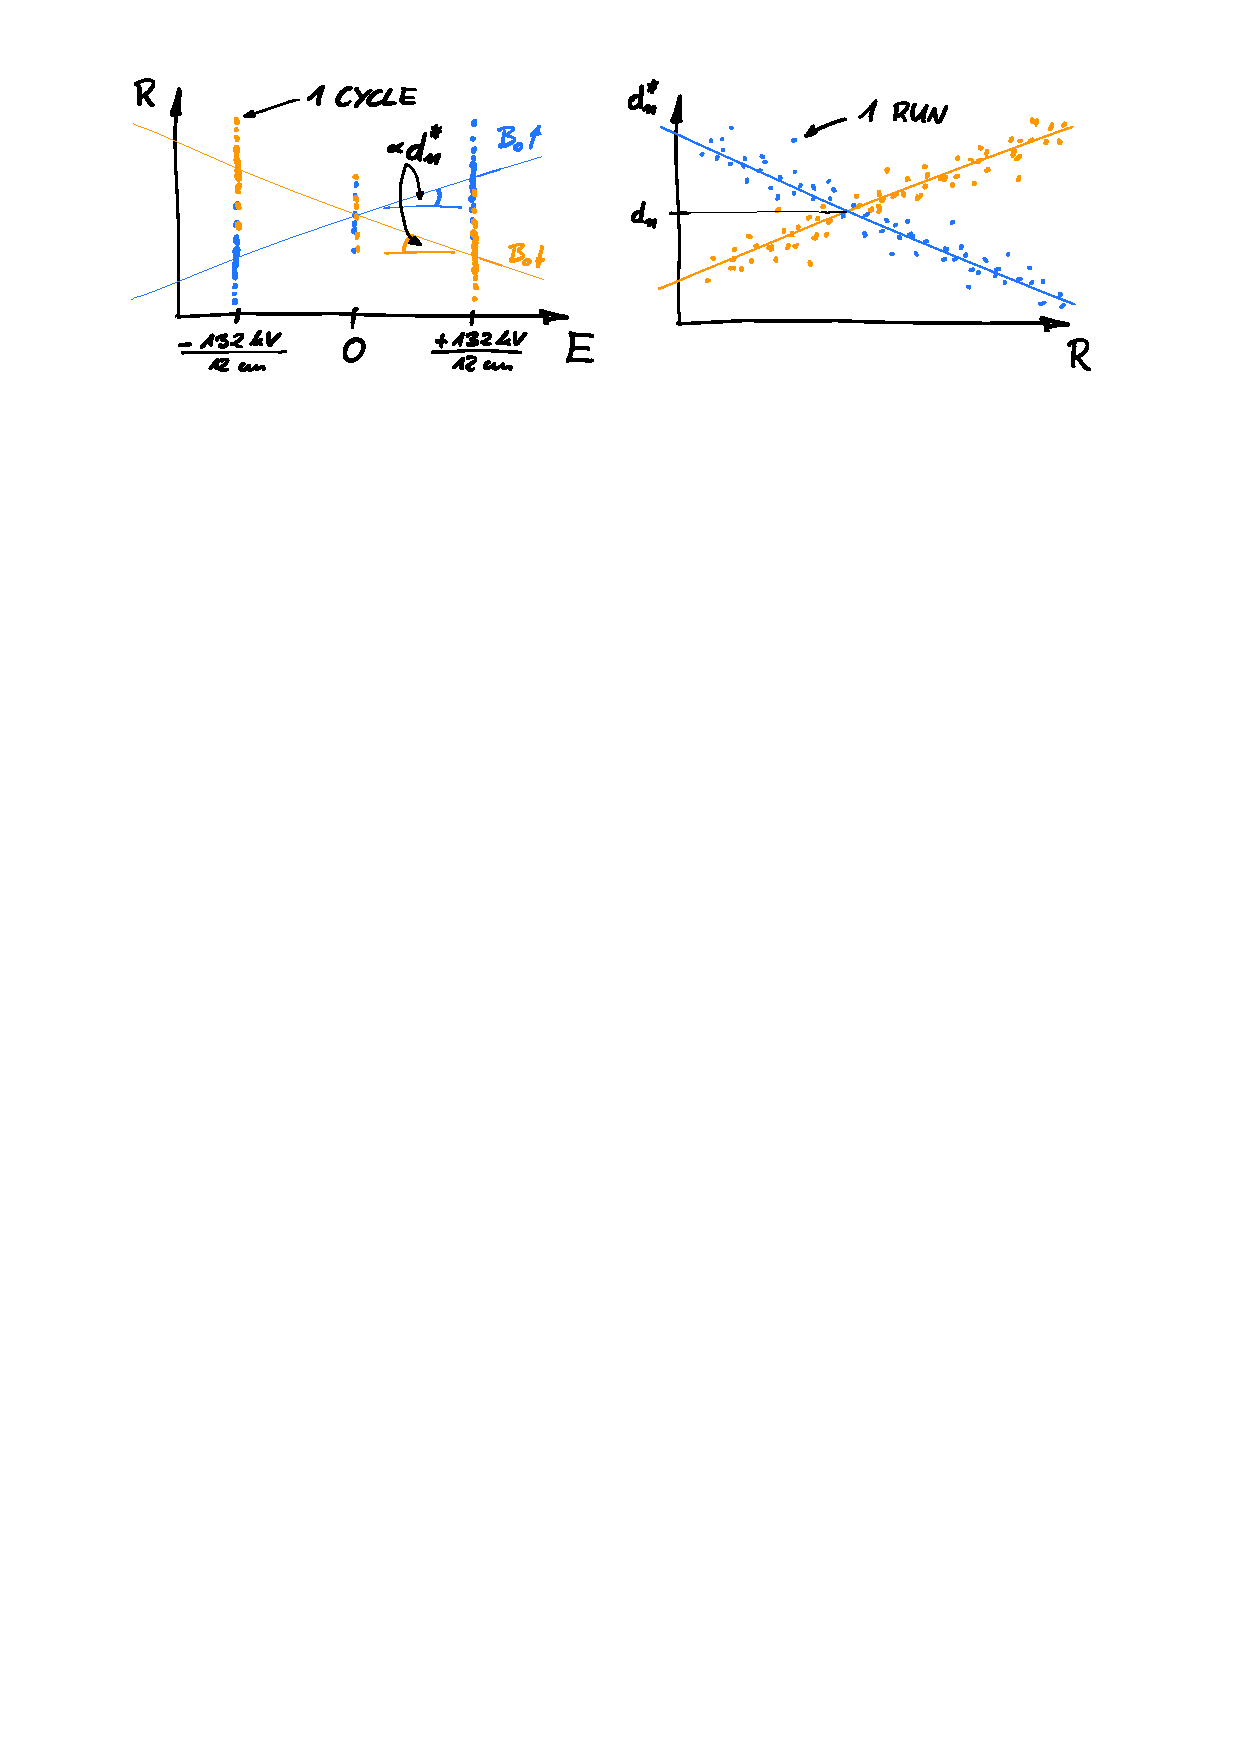
\includegraphics[width=\linewidth]{gfx/nEDMatPSI/crossing_lines.pdf}
  \caption{The crossing lines in the nEDM estimation. Left: For each sequence, data taken in one magnetic field configuration, $d_n^*$ is estimated as the slope of a linear regression of $R$ vs. $E$ (Eq.\,\ref{eq:Rdefinition}). The two lines correspond to the parallel and anti-parallel configurations of the magnetic and electric fields. The $d_n^*$ are tainted by a systematic effect proportional to the gradient. Right: a linear regression is done on $d_n^*$ vs. $R$, $R$ being an estimate of the gradient. The crossing point of the two lines, one for the magnetic field pointing upwards, one for downwards, is the estimate of $d_n$ at zero gradient, so free from the gradient-proportional systematic effect.}\label{fig:crossing_lines}
\end{figure}

Those estimates, however, still contained a large contribution of a systematic effect (hence the star). As a result of a conspiracy between radial magnetic field components and rotating magnetic components arising from the Lorentz transformation of the large electric field into the rest frame of the mercury atoms, a frequency shift proportional to the applied electric field was observed, mimicking the effect of a non-zero electric dipole moment of the neutron, a false EDM\@. This effect is, however, directly proportional to the gradient of the applied vertical magnetic field $\partial_z B_z$, and reverses with the sign of the applied magnetic field. The false EDM effect has been analysed in more detail in~\cite{Pendlebury2004,PhysRevA.71.032104,PhysRevA.73.014101} and a direct measurement of this effect was made in~\cite{Afach2015falseEDM}.

The solution was to operate in different vertical gradients and then interpolate to the effect-free zero gradient. Every few hundred cycles a different gradient (up to $\pm \SI{60}{\pico\tesla\per\centi\meter}$) was set.
%We set the magnetic configuration (homogenise the field, maybe mention the variometer method), apply a gradient (one of i don't remember how many), calibrate the Cs magnetometers (margin note why) and measure continuously cycle after cycle in this configuration.
% We call a set of data taken in one configuration of the magnetic field a \emph{sequence}.
Finally, for each direction of the magnetic field, a linear regression of $d_n^*$ vs $R$, $R$ itself being an estimate of the gradient, was performed (Fig.\,\ref{fig:crossing_lines}). The vertical position of the intersection of the two lines corresponded to the $d_n$ measured at zero gradient, free from this systematic effect.

% In the nEDM experiment at PSI data taking is divided into \emph{runs}. A single \emph{run} is carried out automatically with, in most cases, no human intervention. The machine cycles through the working points by itself. Also the charging of the electrodes creating the electric field is automatised. In between \emph{runs} manual interference happens, most importantly the magnetic field vertical gradient is altered.

\marginpar{The blinding mimicked an nEDM signal
by changing the logged neutron counts by around one neutron each cycle.
by changing the logged detector mark for around one, on average, neutron count. The directon of the change depended on the electric field.}
On top of that, in order to mitigate the bias due to the human factor, the nEDM experiment implemented data blinding. The data was artificially altered in a way that mimicked a non-zero neutron electric dipole moment, big enough to be visible in the data. The exact offset value is secret and would be revealed only after the analysis was complete.

In this short description we only scratched the surface of the quite complex experiment. We discussed only those elements necessary for understanding the original work presented in the next chapters. More details can be found in the following references:~\cite{Zenner2013,Afach2015falseEDM,Afach2015,Afach2014magmoment,FertlThesis,Komposch2017}.
